\documentclass[aspectratio=169,12pt]{beamer}
\usepackage[utf8]{inputenc}
\usepackage{amsmath, amssymb}
\usepackage{booktabs}
\usepackage{colortbl}
\usepackage{hyperref}
\usepackage{makecell}
\usepackage{ragged2e}
\usepackage{tikz}
\usetikzlibrary{arrows.meta, positioning, shapes.geometric, calc, tikzmark, shapes.misc, fit, decorations.pathreplacing}
\usepackage{tcolorbox}
\usepackage{array}
\usetheme{Madrid}

% Custom colors
\definecolor{correctgreen}{RGB}{0,150,0}
\definecolor{incorrectred}{RGB}{200,0,0}
\definecolor{counterblue}{RGB}{70,130,255}
\definecolor{highlightyellow}{RGB}{255,230,100}

\title{Branch Prediction}
\subtitle{Computer Architecture}
\author{Course 234267}
\date{}

\begin{document}

\frame{\titlepage}

%==========================================
\begin{frame}{2-Bit Counter Prediction (Threshold of 2)}
\vspace{-0.3cm}

% \begin{tikzpicture}[
%     every node/.style={font=\footnotesize},
%     pattern/.style={minimum width=0.5cm, minimum height=0.5cm, draw=black!60},
%     predict/.style={minimum width=0.5cm, minimum height=0.5cm, draw=black!60},
%     counter/.style={minimum width=0.5cm, minimum height=0.5cm, draw=counterblue, text=counterblue},
%     correct/.style={fill=correctgreen!20},
%     wrong/.style={fill=incorrectred!30},
%     arrow/.style={->, thick, >=stealth}
% ]

% % Labels
% \node[anchor=east] at (-0.5, 0) {\textbf{Pattern:}};
% \node[anchor=east] at (-0.5, -1) {\textbf{2-bit Prediction:}};
% \node[anchor=east] at (-0.5, -2) {\textbf{Counter:}};

% % Pattern row
% \foreach \i in {0,...,19} {
%     \pgfmathtruncatemacro{\val}{mod(\i,5) < 4 ? 1 : 0}
%     \pgfmathtruncatemacro{\groupnum}{floor(\i/5)}
%     \node[pattern, fill=\val ? white : gray!20] (p\i) at (\i*0.6, 0) {\val};
% }
% \node at (20*0.6, 0) {...};

\begin{tikzpicture}[
    every node/.style={font=\footnotesize},
    pattern/.style={minimum width=0.5cm, minimum height=0.5cm, draw=black!60},
    predict/.style={minimum width=0.5cm, minimum height=0.5cm, draw=black!60},
    counter/.style={minimum width=0.5cm, minimum height=0.5cm, draw=blue},
    correct/.style={fill=green!20},
    wrong/.style={fill=red!30},
    arrow/.style={->, thick, >=stealth}
]

% Labels
\node[anchor=east] at (-0.5, 0) {\textbf{Pattern:}};
\node[anchor=east] at (-0.5, -1) {\textbf{2-bit Prediction:}};
\node[anchor=east] at (-0.5, -2) {\textbf{Counter:}};

% Pattern row
\foreach \i in {0,...,19} {
    \pgfmathtruncatemacro{\val}{mod(\i,5) < 4 ? 1 : 0}
    \pgfmathtruncatemacro{\groupnum}{floor(\i/5)}
    \ifnum\val=1
        \node[pattern, fill=white] (p\i) at (\i*0.6, 0) {\val};
    \else
        \node[pattern, fill=gray!20] (p\i) at (\i*0.6, 0) {\val};
    \fi
}
\node at (20*0.6, 0) {...};

% Prediction row
\pause
\foreach \i in {0,...,19} {
    \node[predict] (pred\i) at (\i*0.6, -1) {1};
}
\node at (20*0.6, -1) {...};

% Counter row
\pause
\foreach \i in {0,...,19} {
    \pgfmathtruncatemacro{\posInGroup}{mod(\i,5)}
    \ifnum\posInGroup=0
        \node[counter, color=blue] (c\i) at (\i*0.6, -2) {2};
    \else
        \ifnum\posInGroup=4
            \node[counter, color=blue] (c\i) at (\i*0.6, -2) {2};
        \else
            \node[counter, color=blue] (c\i) at (\i*0.6, -2) {3};
        \fi
    \fi
}
\node at (20*0.6, -2) {2 3 ...};

% Misprediction indicators
\pause
\foreach \i in {4,9,14,19} {
    % Highlight mispredicted positions
    \node[predict, wrong] at (\i*0.6, -1) {1};
    \draw[red, ultra thick] (p\i.south west) -- (p\i.south east);
    \draw[red, ultra thick] (pred\i.north west) -- (pred\i.north east);
    
    % Add X mark for misprediction
    \node[color=red, font=\Large] at (\i*0.6, -0.5) {$\times$};
}
% Correct prediction indicators (check marks)
\pause
\foreach \i in {0,1,2,3,5,6,7,8,10,11,12,13,15,16,17,18} {
    \node[color=green!60!black, font=\small] at (\i*0.6, -0.5) {$\checkmark$};
}
% Group brackets
\pause
\foreach \g in {0,1,2,3} {
    \pgfmathtruncatemacro{\startx}{\g*5}
    \pgfmathtruncatemacro{\endx}{\g*5+4}
    \pgfmathtruncatemacro{\gnum}{\g+1}
    \draw[decoration={brace,amplitude=5pt,mirror}, decorate, thick, gray] 
        (\startx*0.6-0.25, -2.5) -- (\endx*0.6+0.25, -2.5);
    \node[gray] at (\startx*0.6+1.2, -2.9) {iteration \gnum};
}

\end{tikzpicture}

\vspace{0.3cm}
\pause
\begin{alertblock}{Key Observation}
\centering
\textcolor{incorrectred}{\textbf{2-bit counter $\rightarrow$ one misprediction every iteration}}
\end{alertblock}

\pause
\vspace{0.2cm}
\begin{block}{Performance Example}
\begin{columns}[T]
\column{0.55\textwidth}
\begin{itemize}
\item<8-> Assume 1 of 20 branches mispredicts\\
      \textcolor{gray}{\small (19 predictions are correct)}
\item<9-> Branch frequency: 20\%\\
      \textcolor{gray}{\small (1 of 5 instructions is branch)}
\item<10-> \textcolor{incorrectred}{\textbf{$\rightarrow$ 1 mispredict every 100 instructions}}
\end{itemize}

\column{0.45\textwidth}
\begin{itemize}
\item<11-> IPC without penalty = 2\\
      \textcolor{gray}{\small (two instructions finish per cycle)}
\item<12-> Mispredict penalty: 10 cycles
\item<13-> \textcolor{incorrectred}{\textbf{$\rightarrow$ 1 mispredict every 50 cycles}}
\item<14-> \textcolor{incorrectred}{\textbf{$\rightarrow$ 10 cycles penalty every 50 cycles}}
\end{itemize}
\end{columns}

\vspace{0.3cm}
\visible<15->{
\begin{tcolorbox}[colback=red!10, colframe=red!60, boxrule=2pt]
\centering
\Large \textcolor{incorrectred}{\textbf{$\rightarrow$ 20\% performance loss!}}
\end{tcolorbox}
}
\end{block}

\end{frame}

\begin{frame}{Better Idea: Use Branch History}

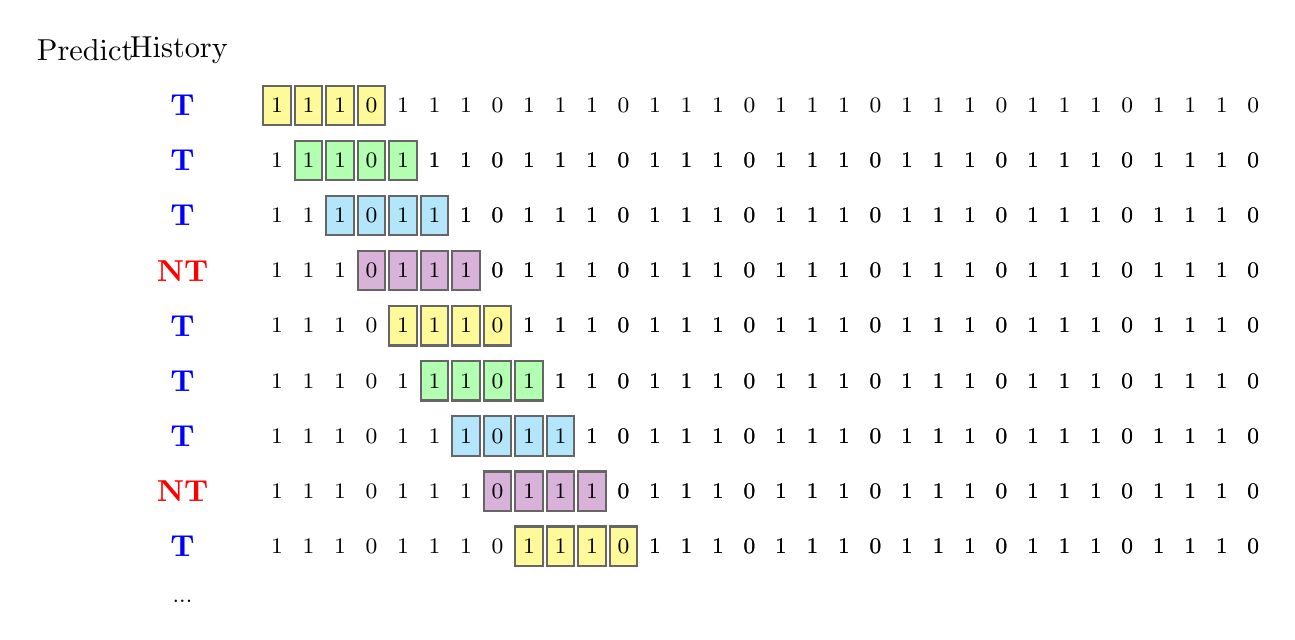
\begin{tikzpicture}[
    every node/.style={font=\footnotesize},
    bit/.style={minimum width=0.35cm, minimum height=0.5cm, inner sep=1pt},
    history1110/.style={bit, draw=black!60, fill=yellow!40, thick},
    history1101/.style={bit, draw=black!60, fill=green!30, thick},
    history1011/.style={bit, draw=black!60, fill=cyan!30, thick},
    history0111/.style={bit, draw=black!60, fill=violet!30, thick},
    predict/.style={font=\fontsize{11}{13}\selectfont\bfseries}
]

% Labels
\node[anchor=east, font=\fontsize{11}{13}\selectfont] at (-1.2, 0) {Predict};
\node[anchor=east, font=\fontsize{11}{13}\selectfont] at (0, 0) {History};

% Pattern template (repeated pattern: 11101110...)
\def\patternseq{1,1,1,0,1,1,1,0,1,1,1,0,1,1,1,0,1,1,1,0,1,1,1,0,1,1,1,0,1,1,1,0}

% Row 1 - History: 1110 -> Predict T
\node[predict, text=blue] at (-0.7, -0.7) {T};
\foreach \i in {0,...,31} {
    \pgfmathparse{{\patternseq}[\i]}
    \pgfmathtruncatemacro{\val}{\pgfmathresult}
    \ifnum\i<4
        \node[history1110] at (\i*0.4 + 0.5, -0.7) {\val};
    \else
        \node[bit] at (\i*0.4 + 0.5, -0.7) {\val};
    \fi
}

% Row 2 - History: 1110 -> Predict T
\node[predict, text=blue] at (-0.7, -1.4) {T};
\foreach \i in {0,...,31} {
    \pgfmathparse{{\patternseq}[\i]}
    \pgfmathtruncatemacro{\val}{\pgfmathresult}
    \ifnum\i>0 \ifnum\i<5
        \node[history1101] at (\i*0.4 + 0.5, -1.4) {\val};
    \else
        \node[bit] at (\i*0.4 + 0.5, -1.4) {\val};
    \fi \fi
    \ifnum\i=0
        \node[bit] at (\i*0.4 + 0.5, -1.4) {\val};
    \fi
    \ifnum\i>4
        \node[bit] at (\i*0.4 + 0.5, -1.4) {\val};
    \fi
}

% Row 3 - History: 1101 -> Predict T  
\node[predict, text=blue] at (-0.7, -2.1) {T};
\foreach \i in {0,...,31} {
    \pgfmathparse{{\patternseq}[\i]}
    \pgfmathtruncatemacro{\val}{\pgfmathresult}
    \ifnum\i>1 \ifnum\i<6
        \node[history1011] at (\i*0.4 + 0.5, -2.1) {\val};
    \else
        \node[bit] at (\i*0.4 + 0.5, -2.1) {\val};
    \fi \fi
    \ifnum\i<2
        \node[bit] at (\i*0.4 + 0.5, -2.1) {\val};
    \fi
    \ifnum\i>5
        \node[bit] at (\i*0.4 + 0.5, -2.1) {\val};
    \fi
}

% Row 4 - History: 1011 -> Predict NT
\node[predict, text=red] at (-0.7, -2.8) {NT};
\foreach \i in {0,...,31} {
    \pgfmathparse{{\patternseq}[\i]}
    \pgfmathtruncatemacro{\val}{\pgfmathresult}
    \ifnum\i>2 \ifnum\i<7
        \node[history0111] at (\i*0.4 + 0.5, -2.8) {\val};
    \else
        \node[bit] at (\i*0.4 + 0.5, -2.8) {\val};
    \fi \fi
    \ifnum\i<3
        \node[bit] at (\i*0.4 + 0.5, -2.8) {\val};
    \fi
    \ifnum\i>6
        \node[bit] at (\i*0.4 + 0.5, -2.8) {\val};
    \fi
}

% Row 5 - History: 0111 -> Predict T
\node[predict, text=blue] at (-0.7, -3.5) {T};
\foreach \i in {0,...,31} {
    \pgfmathparse{{\patternseq}[\i]}
    \pgfmathtruncatemacro{\val}{\pgfmathresult}
    \ifnum\i>3 \ifnum\i<8
        \node[history1110] at (\i*0.4 + 0.5, -3.5) {\val};
    \else
        \node[bit] at (\i*0.4 + 0.5, -3.5) {\val};
    \fi \fi
    \ifnum\i<4
        \node[bit] at (\i*0.4 + 0.5, -3.5) {\val};
    \fi
    \ifnum\i>7
        \node[bit] at (\i*0.4 + 0.5, -3.5) {\val};
    \fi
}

% Row 6 - History: 1110 -> Predict T
\node[predict, text=blue] at (-0.7, -4.2) {T};
\foreach \i in {0,...,31} {
    \pgfmathparse{{\patternseq}[\i]}
    \pgfmathtruncatemacro{\val}{\pgfmathresult}
    \ifnum\i>4 \ifnum\i<9
        \node[history1101] at (\i*0.4 + 0.5, -4.2) {\val};
    \else
        \node[bit] at (\i*0.4 + 0.5, -4.2) {\val};
    \fi \fi
    \ifnum\i<5
        \node[bit] at (\i*0.4 + 0.5, -4.2) {\val};
    \fi
    \ifnum\i>8
        \node[bit] at (\i*0.4 + 0.5, -4.2) {\val};
    \fi
}

% Row 7 - History: 1101 -> Predict T
\node[predict, text=blue] at (-0.7, -4.9) {T};
\foreach \i in {0,...,31} {
    \pgfmathparse{{\patternseq}[\i]}
    \pgfmathtruncatemacro{\val}{\pgfmathresult}
    \ifnum\i>5 \ifnum\i<10
        \node[history1011] at (\i*0.4 + 0.5, -4.9) {\val};
    \else
        \node[bit] at (\i*0.4 + 0.5, -4.9) {\val};
    \fi \fi
    \ifnum\i<6
        \node[bit] at (\i*0.4 + 0.5, -4.9) {\val};
    \fi
    \ifnum\i>9
        \node[bit] at (\i*0.4 + 0.5, -4.9) {\val};
    \fi
}

% Row 8 - History: 1011 -> Predict NT
\node[predict, text=red] at (-0.7, -5.6) {NT};
\foreach \i in {0,...,31} {
    \pgfmathparse{{\patternseq}[\i]}
    \pgfmathtruncatemacro{\val}{\pgfmathresult}
    \ifnum\i>6 \ifnum\i<11
        \node[history0111] at (\i*0.4 + 0.5, -5.6) {\val};
    \else
        \node[bit] at (\i*0.4 + 0.5, -5.6) {\val};
    \fi \fi
    \ifnum\i<7
        \node[bit] at (\i*0.4 + 0.5, -5.6) {\val};
    \fi
    \ifnum\i>10
        \node[bit] at (\i*0.4 + 0.5, -5.6) {\val};
    \fi
}

% Row 9 - History: 0111 -> Predict T
\node[predict, text=blue] at (-0.7, -6.3) {T};
\foreach \i in {0,...,31} {
    \pgfmathparse{{\patternseq}[\i]}
    \pgfmathtruncatemacro{\val}{\pgfmathresult}
    \ifnum\i>7 \ifnum\i<12
        \node[history1110] at (\i*0.4 + 0.5, -6.3) {\val};
    \else
        \node[bit] at (\i*0.4 + 0.5, -6.3) {\val};
    \fi \fi
    \ifnum\i<8
        \node[bit] at (\i*0.4 + 0.5, -6.3) {\val};
    \fi
    \ifnum\i>11
        \node[bit] at (\i*0.4 + 0.5, -6.3) {\val};
    \fi
}

% ... dots
\node at (-0.7, -7) {...};

\end{tikzpicture}

\end{frame}

%==========================================
% Add more slides here as needed

\end{document}